In this chapter, we will discuss the background on how sponsored search works followed by the notion of coverage patterns, which is the key pillar in the proposed approaches.



\section{Sponsored Search Framework}
In sponsored search, an advertiser has a daily budget and bids on a set of keywords. For every query that is fired, the set of advertisers who have bid upon any keywords contained in the query are ranked on the basis of their bids and top-k advertisers are chosen to be displayed as the sponsored results.

\begin{figure}[h]
	\centering
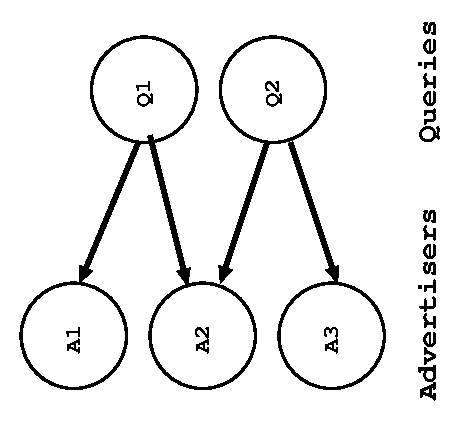
\includegraphics[scale=0.55,angle = 270]{visuals/present_model.eps}
	\caption{Sponsored Search Model}
	\label{fig:adwords:model}
\end{figure}


Mehta {\it et al.} \cite{mehta2007adwords} framed the problem of sponsored search as a bipartite matching problem. An instance of the same is shown in Figure \ref{fig:adwords:model}. In this model, the left side is the set of advertisers and the right side is the set of incoming queries which are to be matched to the advertisers. When a query is fired by a user, it is to be matched to the relevant advertisers. The advertisers are then ranked and their advertisements are displayed along with query results.

Figure \ref{fig:adwords:architecture} shows the framework of sponsored search by considering single query as an input and a list of candidate advertisers to be displayed with the results as the output. The framework contains the following steps.


\begin{enumerate}[label=(\roman*).]
\item {\em Analysis of Query}: In this part, a search query is analyzed for the purpose of identification of information which is useful for showing advertisements on search results page. This information could be in form of topic of the query, previous queries in the session and topics explored in the session apart from several other parameters.
\item {\em Retrieval of Relevant Advertisers}: In this step, relevant advertisements are retrieved from the created ad campaigns. This is performed by employing  appropriate  similarity measures between  the bid keywords and the query keywords.
\item{\em Bidding}: Due to competition among advertisers, incoming queries are allotted to advertisers through auctions such that advertisers bid for placing their ads on the query's results page. These bids can either be static or can be done in real time.
\item{\em Ranking of Advertisers}: Once the advertisers bid on a query, their bids are scaled according to a factor called {\it Quality Score}. {\it Quality Score} is computed based on the parameters related to the respective advertisement. This includes expected {\it CTR (Click Through Rate)}, display URL's past {\it CTR}, quality of the landing page, remaining budget and ad-query relevance apart from several other parameters \cite{qualityScore}.
\end{enumerate}
\begin{figure*}
	\centering
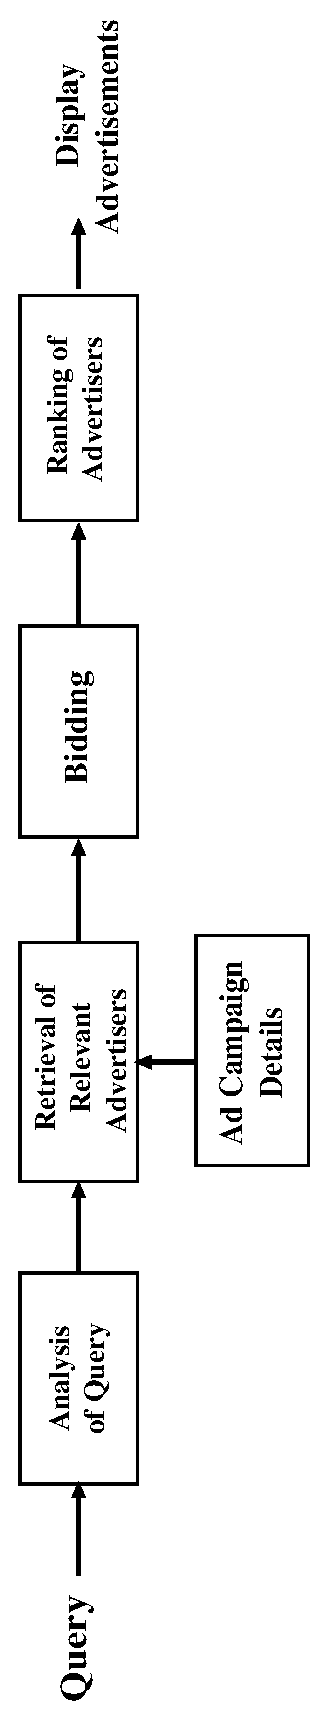
\includegraphics[scale=0.55,angle = 270]{visuals/present.eps}
	\caption{Sponsored Search Architecture as discussed in \cite{mehta2007adwords}}
	\label{fig:adwords:architecture}
\end{figure*}


\section{Overview of Coverage Patterns Model} 
\label{sec:CoveragePatternsModel}
The model of coverage patterns was proposed in \cite{sripada2011coverage, srinivas2014mining} for efficient banner advertising. The click-through data of a website represents the navigational patterns of multiple visitors. The model of coverage patterns is used to mine these click-stream logs to extract interesting combination of web pages for advertising. Let $W=\{w_1,w_2,w_3\cdots,w_n\}$ be the set of web page identifiers and $D$ is the set of transactions, where each transaction T is the set of web pages such that $T \subseteq W$. A set of web pages $X \subseteq W$ i.e., $X=\{w_p,\cdots,w_q,w_r\}, 1\leq p \leq q \leq r \leq n$ is a pattern. Every web page $w_i$ is related to multiple topics, $\{tp_1,tp_2,tp_3,\cdots tp_m\}$, where $m$ is the number of topics in $w_i$. Set of transactions containing web page $w_i$ is denoted as $T^{w_i}$ and its cardinality is denoted as $|T^{w_i}|$.  Transactional database, $D$ is given in Table \ref{tb:transactionalDatabase}.
	
\begin{table}[ht]\centering
\renewcommand{\arraystretch}{1.3}
\caption{Transactional database, D}
\label{tb:transactionalDatabase}
\begin{tabular}{|l|l|l|l|l|l|l|l|l|l|l|l|}
%\begin{tabular}{|p{0.4cm}|p{0.4cm}|p{0.4cm}|p{0.4cm}|p{0.4cm}|p{0.4cm}|p{0.4cm}|p{0.4cm}|p{0.4cm}|p{0.4cm}|p{0.2cm}|}
\hline
TID & 1 & 2 & 3 & 4 & 5 & 6 & 7 & 8 & 9 & 10 \\
\hline
Web pages & b, a, c & a, c, e & a, c, e & a, c, d & b, d, f & b, d & b, d & b, e & b, e & b, a \\
\hline
\end{tabular}
\end{table}
	Web pages are said to be potential web pages for placing advertisement when they occur in more number of transactions. This means that web pages are having more number of visitors. This is captured by the aspect of \emph{relative frequency}.  

\begin{mydef}
(Relative frequency (RF)) and Frequent web page)  The RF of a web page  $w_i$,  denoted by  $RF(w_i)$, is equal to the ratio of number of transactions that contain $w_i$ to D, i.e., $RF(w_i) = \frac{|T^{w_i}|}{|D|}$. Let the term `minimum relative frequency (minRF)' indicate user-specified threshold value. A web page is frequent if it is no less than minimum threshold frequency, $minRF$, i.e., RF($w_i$) $\geq$ $minRF$. 
\end{mydef}
	
	Given a pattern, it is interesting to find the users visiting at least one of the web pages in the pattern. It is interesting because if we place the advertisement on all the web pages in the pattern, it guarantees the delivery of the advertisement to the users visiting at least one of the web pages in the pattern. This is captured by the aspect of \emph{coverage set}.

\begin{mydef} \label{csup}
(Coverage set and \emph{coverage support (CS)} of a pattern $X = \{w_p, \cdots$ $,w_q, w_r\}$, $1\leq p, q, r \leq n$) The set of distinct transaction ids containing at least one web page of $X$ is called coverage set of pattern $X$ and is denoted as $CSet(X)$. Therefore, $CSet(X) = T^{w_p}\cup \cdots  \cup T^{w_q} \cup T^{w_r}$. The ratio of the size of the $CSet(X)$ to $D$ is called the coverage-support of pattern $X$ and is denoted as $CS(X)$, i.e., $CS(X) = \frac{|CSet(X)|}{|D|}$.
\end{mydef}
	
	Given a pattern, adding a new item which co-occur with any of the items in the dataset may not increase the coverage support significantly. This is not interesting from the banner advertisement perspective as the same user is visiting these web pages having same advertisement. The new pattern formed by adding the new item is interesting it there is minimum overlap between the \emph{coverage sets} of web pages. This is captured by the aspect of \emph{overlap-ratio}.
	 
\begin{mydef}
(Overlap ratio (OR) of a pattern.) OR of a pattern $X=\{w_p,\cdots$ $,w_q,w_r\}$, where $1\leq p, q, r \leq n$ and $|T^{w_p}|\geq\cdots \geq |T^{w_{q}}| \geq |T^{w_{r}}| $, is the ratio of the number of transactions common in $X-\{w_r\}$ and $\{w_r\}$ to the number of transactions in $w_r$, i.e., $OR(X) = \frac{|(Cset(X-\{w_r\})) \cap (Cset\{w_r\})|} {|Cset\{w_r\}|}$.
\label{overLap}
\end{mydef}
	The items in the pattern are ordered in descending order of frequency to satisfy the property of \emph{sorted downward closure property} which is later helpful in mining coverage patterns.
	   
	 A pattern X is said to be \emph{non-overlap pattern} if $OR(X)$ is no greater than $maxOR$ and $ \forall w_i \in X$, $RF(w_i) \geq minRF$. An item `a' is said to be \emph{non-overlap item} with respect to $X$, if $OR({X,a})$ is no greater than $maxOR$.
	
	A \emph{coverage pattern} is said to be interesting if it has high $CS$ and low $OR$. It is interesting because having high $CS$ means showing the advertisement to many users and having low $OR$ means decreasing the repetitive display of advertisement. i.e., a pattern $X$ is said to be interesting if $CS(X) \geq minCS$, $OR(X) \leq maxOR$, and $RF(w_i) \geq minRF$ $\forall w_i \in X$. A coverage pattern $X$ having $CS(X)=a\%$ and $OR(X)=b\%$ is denoted as follows:
\begin{eqnarray}
\label{coveragePattern}
X~~~[CS=a\%, ~ OR=b\%] \nonumber
\end{eqnarray}

\begin{myexp}
\label{ex:coveragePatternExample}
From Table \ref{tb:transactionalDatabase}, the relative frequency of `$a$' i.e., $RF(a)=\frac{|T^{a}|}{|D|}=\frac{5}{10}=0.5$. If the user-specified $minRF=0.5$, then `$a$' is called a frequent web page because $RF(a) \geq minRF$. Similarly for `$b$' relative frequency is  $RF(b)=\frac{|T^{b}|}{|D|}=\frac{7}{10}=0.7$. `$b$' is called a frequent web page because $RF(b) \geq minRF$. The set of web pages `$a$' and `$b$' i.e., $\{a,b\}$ is a pattern. The set of $TIDs$ containing the web page `$a$' i.e., $T^{a} =\{1, 2, 3, 4, 10\}$. Similarly, $T^{b}=\{1, 5, 6, 7, 8, 9, 10\}$. The coverage set of $\{a,b\}$ i.e., $CSet(\{a,b\}) = \{1, 2, 3, 4, 5, 6, 7, 8, 9, 10\} $. Therefore, coverage support of $\{a,b\}$ i.e., $ CS(\{a,b\}) = \frac{|CSet(\{a,b\})|}{|D|} = \frac{10}{10}=1$.  The $OR(\{a,b\}) = \frac{|CSet(b) \cap CSet(a)|}{|CSet(a)|} = \frac{2}{10} = 0.2$. If $minRF=0.4$, $minCS=0.7$ and $maxOR=0.5$, then the pattern $\{a,b\}$ is a coverage pattern. It is because $RF(a) \geq minRF$, $RF(b) \geq minRF$, $CS(\{a,b\}) \geq minCS$ and $OR(\{a,b\}) \leq maxOR$. This pattern is written as follows:
\begin{eqnarray}
\{a,b\} ~~~[CS=1 ~(=100\%), ~OR= 0.1~(=10\%)] \nonumber
\end{eqnarray}
\end{myexp}

In this rest of this section, we first give an overview of the approaches proposed for extracted coverage patterns followed by an overview of the CMine algorithm.

	
\subsection{Overview of approaches to mine Coverage Patterns}
\label{sec:CovPatternMining}
The problem statement of mining coverage patterns is as follows. Given a transactional database $D$, set of web pages $W$ (or items), and the user-specified \emph{minimum relative frequency} ($minRF$), \emph{minimum coverage support} ($minCS$) and \emph{maximum overlap ratio} ($maxOR$), discover the complete set of coverage patterns in the database that satisfy \emph{minRF}, \emph{minCS} and \emph{maxOR} thresholds. A naive approach is exponential because for a given website of `n' web pages, we have to check for $minCS$ and $maxOR$ for all $(2^n-1)$ sets of web pages. 

An Apriori like approach, \emph{CMine} which is based on multiple pass, candidate test and generation approach is proposed in \cite{srinivas2012discovering}. It uses the fact that every non-overlap pattern is coverage pattern and by using the sorted closure property of overlap ratio the search space is minimized. Later, a pattern-growth approach, \emph{coverage pattern projected growth (CPPG)} based on the notion of \emph{non-overlap projection} is proposed in \cite{srinivas2013cppg}. An enhanced coverage pattern projected growth approach, \emph{ECPPG} is proposed in \cite{srinivas2014mining} by using the notion of \emph{upward closure property} of coverage patterns.

The overview of \emph{CMine} algorithm is as follows. 

\subsection{ CMine Algorithm with Example}
\label{subsec:cmine}
 Let $F$ be a set of frequent items, $C_k$ be a set of candidate k-patterns, $L_k$ be a set of coverage k-patterns and $NO_k$ be a set of non-overlap k-patterns.  The algorithm \emph{CMine} begins with a scan of database and discovers set of all frequent web pages (denoted as F) and coverage 1-patterns (denoted as $C_1$). Non-overlap patterns (denoted as $NO_1$) will be the set of all frequent 1 items. Next, the items in $NO_1$ are sorted in descending order of their frequencies. Using $NO_1$ as the seed set, candidate patterns $C_2$ are generated by combining $NO_1 \Join NO_1$. From $C_2$, the patterns that satisfy $minCS$ and $maxOR$ are generated as  $L_2$. Simultaneously, all candidate 2-patterns that satisfy $maxOR$ constraints are generated as non-overlap 2-patterns, $NO_2$. Since \emph{overlap ratio} satisfies sorted closure property, $C_3$ is generated by combining $NO_2 \Join NO_2$. This process is repeated until no new coverage patterns are found or no new candidate patterns can be generated.
The proposed algorithm uses bitwise OR and AND operations to find the \emph{coverage support} and \emph{overlap ratio}  of a pattern, respectively.  So, single scan of database is sufficient to find the bit strings of all single web pages and to extract the complete set of coverage patterns.

\begin{figure*}[htp]\centering
\centerline {\includegraphics[height=0.4\textwidth, width=0.8\textwidth, natwidth=800, natheight=400]{visuals/CMine.jpg}}
\caption{Working of CMine algorithm. The term `I' is an acronym for the item set (or web pages).} \label{AprioriAlgorithm}
\end{figure*}
We now explain the working of \emph{CMine} algorithm using the transactional database, $D$, shown in Table \ref{tb:transactionalDatabase} for the user-specified $minRF$, $minCS$ and $maxOR$ as 0.4, 0.7 and 0.5, respectively. We use Figure \ref{AprioriAlgorithm} to illustrate the \emph{CMine} algorithm for finding coverage patterns in $D$.

The algorithm \emph{CMine} scans all the transactions to generate bit string $|B^{w_i}|$ and relative frequencies ($RF$) of each web page $w_i$. $RF(w_i) = \frac{|B^{w_i}|}{|T|}$. $|B^{w_i}|$ denotes the number of 1's in the bit string. Each web page, $w_i$  $\epsilon$ $T$ which has a relative frequency no less than 0.4 is a member of the set of candidate 1-pattern, $C_1$. From $C_1$, the set of coverage 1-patterns, $L_1$, are discovered if their frequencies are greater than or equal to $minCS$. Simultaneously, set of non-overlap 1-patterns, $NO_1$, are discovered if candidate 1-patterns have relative support greater than or equal to $minRF$ and finally the web pages in $NO_1$ are sorted in the decreasing order of their frequencies. To discover the set of coverage 2-patterns, $L_2$, the algorithm computes the join of $NO_1 \Join NO_1$ to generate a candidate set of 2-patterns, $C_2$. Next, \emph{overlap ratio} and \emph{coverage ratio} for each candidate pattern is computed. \emph{Coverage support} is computed by boolean OR operation and \emph{overlap ratio} is computed by boolean AND operation. For example, $CS(\{b,a\}) = \frac{|B^b \lor B^a|}{|T|} = \frac{|1111111111|}{10} = 1.0$ and $OR(\{b,a\}) = \frac{|B^b \land B^a|}{|B^a|} = \frac{|10000001|}{10} = \frac{2}{10} = 0.4$.

  The columns titled `$CS$' and `$OR$' respectively show the \emph{coverage support} and \emph{overlap ratio} for the patterns. The set of candidate 2-patterns that satisfy $maxOR$ are discovered as non-overlap 2-patterns, denoted as $NO_2$. Simultaneously, the set of candidate 2-patterns that satisfy both $minCS$ and $maxOR$ are discovered as coverage 2-patterns. Next, $C_3$ is generated by $NO_2 \Join NO_2$. We discover non-overlap 3-patterns, $NO_3$, and coverage 3-patterns, $L_3$ in the same manner that is stated above. The algorithm stops as no more candidate 4-patterns can be generated from non-overlap 3-patterns.


\section{Summary}
\label{sec:Summary3}
In this chapter, we discuss how sponsored search works followed by an overview of coverage patterns. We discussed the model of coverage patterns followed by approaches to extract coverage patterns. Cmine approach was discussed in detail. 